% ==========================================================================
% Rapport final du projet RADAR
% Module M244 - Veille Technologique
% ENSA Tetouan - Cycle Ingenieur BDIA - Printemps 2026
% Auteurs : Bachirou Konate et Karamo Sylla
% Encadrant : Pr. Younes Wadiai
% ==========================================================================

\documentclass[12pt,a4paper,openany]{report}

% --- Encodage et langue ---------------------------------------------------
\usepackage[utf8]{inputenc}
\usepackage[T1]{fontenc}
\usepackage[french]{babel}
\usepackage{lmodern}

% --- Mise en page ---------------------------------------------------------
\usepackage[a4paper,top=2.5cm,bottom=2.5cm,left=3cm,right=2.5cm]{geometry}
\usepackage{setspace}
\onehalfspacing

% --- Couleurs ENSA --------------------------------------------------------
\usepackage{xcolor}
\definecolor{ensaBlue}{HTML}{002C5F}
\definecolor{ensaBlueLight}{HTML}{1F4E8C}
\definecolor{ensaAccent}{HTML}{D97706}
\definecolor{grayBox}{HTML}{F4F4F5}
\definecolor{grayBorder}{HTML}{D4D4D8}

% --- Polices titres -------------------------------------------------------
\usepackage{titlesec}
\titleformat{\chapter}[display]
  {\normalfont\sffamily\Huge\bfseries\color{ensaBlue}\raggedright}
  {\sffamily\huge\color{ensaBlueLight}Chapitre \thechapter}
  {1ex}
  {\titlerule\vspace{1ex}\raggedright}
  [\vspace{0.5ex}\titlerule]
\titlespacing*{\chapter}{0pt}{-30pt}{20pt}
\titleformat{\section}
  {\normalfont\sffamily\Large\bfseries\color{ensaBlue}}
  {\thesection}{1em}{}
\titleformat{\subsection}
  {\normalfont\sffamily\large\bfseries\color{ensaBlueLight}}
  {\thesubsection}{1em}{}
\titleformat{\subsubsection}
  {\normalfont\sffamily\normalsize\bfseries\color{ensaBlueLight}}
  {\thesubsubsection}{1em}{}

% --- Graphiques et figures ------------------------------------------------
\usepackage{graphicx}
\graphicspath{{images/}}
\usepackage{float}
\usepackage{caption}
\captionsetup{font=small,labelfont={bf,color=ensaBlue},labelsep=period}
\usepackage{tikz}
\usetikzlibrary{shapes,arrows,positioning,fit,backgrounds,calc}

% --- Tableaux -------------------------------------------------------------
\usepackage{booktabs}
\usepackage{tabularx}
\usepackage{multirow}
\usepackage{array}
\usepackage{colortbl}
\newcolumntype{Y}{>{\raggedright\arraybackslash}X}

% --- Code source ----------------------------------------------------------
\usepackage{listings}
\lstdefinestyle{radarstyle}{
  backgroundcolor=\color{grayBox},
  basicstyle=\ttfamily\footnotesize,
  keywordstyle=\color{ensaBlue}\bfseries,
  commentstyle=\color{gray}\itshape,
  stringstyle=\color{ensaAccent},
  numbers=left,
  numberstyle=\tiny\color{gray},
  numbersep=8pt,
  frame=single,
  rulecolor=\color{grayBorder},
  breaklines=true,
  showstringspaces=false,
  tabsize=2,
  captionpos=b
}
\lstset{style=radarstyle}

% --- Encadres personnalises -----------------------------------------------
\usepackage[most]{tcolorbox}
\newtcolorbox{noteBox}[1][]{
  colback=grayBox,
  colframe=ensaBlueLight,
  fonttitle=\bfseries\sffamily\color{white},
  coltitle=white,
  colbacktitle=ensaBlueLight,
  title=Note,
  sharp corners,
  boxrule=0.5pt,
  #1
}
\newtcolorbox{decisionBox}[1][]{
  colback=grayBox,
  colframe=ensaAccent,
  fonttitle=\bfseries\sffamily\color{white},
  coltitle=white,
  colbacktitle=ensaAccent,
  title=Decision technique,
  sharp corners,
  boxrule=0.5pt,
  #1
}

% --- En-tetes et pieds de page --------------------------------------------
\usepackage{fancyhdr}
\pagestyle{fancy}
\fancyhf{}
\fancyhead[L]{\small\sffamily\color{ensaBlueLight}\nouppercase{\leftmark}}
\fancyhead[R]{\small\sffamily\color{ensaBlueLight}RADAR · M244}
\fancyfoot[C]{\thepage}
\renewcommand{\headrulewidth}{0.4pt}
\renewcommand{\footrulewidth}{0pt}

% --- Listes ---------------------------------------------------------------
\usepackage{enumitem}
\setlist{itemsep=2pt,topsep=4pt}

% --- Mise en colonnes pour la bibliographie -------------------------------
\usepackage{multicol}

% --- Liens et bibliographie ------------------------------------------------
\usepackage{hyperref}
\hypersetup{
  colorlinks=true,
  linkcolor=ensaBlue,
  urlcolor=ensaAccent,
  citecolor=ensaBlue,
  pdftitle={RADAR - Rapport final M244},
  pdfauthor={Bachirou Konate, Karamo Sylla},
  pdfsubject={Veille Technologique - ENSA Tetouan},
  bookmarksopen=true
}
\usepackage[french]{cleveref}

% --- Commande pour les figures a inserer plus tard ------------------------
\newcommand{\figurePlaceholder}[2]{%
  \begin{figure}[H]
    \centering
    \fbox{\parbox[c][4cm][c]{0.85\linewidth}{\centering\sffamily\color{gray}\itshape #2}}
    \caption{#1}
  \end{figure}
}

\begin{document}

% =========================================================================
% PAGE DE GARDE
% =========================================================================
\begin{titlepage}
  \centering
  \vspace*{-3cm}

  % Logo ENSA agrandi et colle au bord superieur
  
\includegraphics[height=8cm]{logo_ensa.png}

  \vspace{-0.3cm}

  % Filets bleus encadrant les informations academiques (texte agrandi)
  {\color{ensaBlue}\rule{\linewidth}{1.2pt}}\\[10pt]
  {\sffamily\large\color{ensaBlue}\textbf{Cycle Ingenieur en Big Data et Intelligence Artificielle (BDIA)}}\\[5pt]
  {\sffamily\large\color{ensaBlueLight}Module M244 \; $\bullet$ \; Veille Technologique}\\[10pt]
  {\color{ensaBlue}\rule{\linewidth}{1.2pt}}

  \vspace{0.4cm}

  % Etiquette discrete au-dessus du titre
  {\sffamily\large\color{ensaBlueLight}\itshape Rapport de projet de fin de module}

  \vspace{0.8cm}

  % Titre principal dans un bloc bleu accentue, centre verticalement
  \begin{tcolorbox}[
    enhanced,
    colback=ensaBlue,
    colframe=ensaBlue,
    sharp corners,
    boxrule=0pt,
    left=15pt, right=15pt, top=28pt, bottom=28pt,
    width=\linewidth,
    drop fuzzy shadow=ensaBlueLight,
  ]
    \centering
    {\sffamily\fontsize{52}{56}\selectfont\bfseries\color{white} RADAR}\\[14pt]
    {\color{ensaAccent}\rule{4cm}{1pt}}\\[14pt]
    {\sffamily\Large\color{white} Plateforme de veille concurrentielle autonome}\\[6pt]
    {\sffamily\Large\color{white} propulsee par un agent IA}
  \end{tcolorbox}

  \vfill

  % Equipe et encadrant en deux colonnes
  \noindent
  \begin{minipage}[t]{0.48\linewidth}
    \raggedright\sffamily
    {\large\color{ensaBlue}\textbf{Realise par}}\\[4pt]
    {\color{ensaAccent}\rule{2.5cm}{1pt}}\\[8pt]
    \large KONATE BACHIROU\\[2pt]
    \large SYLLA KARAMO
  \end{minipage}\hfill
  \begin{minipage}[t]{0.48\linewidth}
    \raggedleft\sffamily
    {\large\color{ensaBlue}\textbf{Encadre par}}\\[4pt]
    {\color{ensaAccent}\rule{2.5cm}{1pt}}\\[8pt]
    \large Pr. Younes WADIAI
  \end{minipage}

  \vspace{1cm}

  % Annee universitaire dans un filet discret
  {\color{ensaBlueLight}\rule{0.4\linewidth}{0.4pt}}\\[8pt]
  {\sffamily\large\color{ensaBlue}\textbf{Annee universitaire 2025 -- 2026}}

\end{titlepage}

% =========================================================================
% REMERCIEMENTS
% =========================================================================
\chapter*{Remerciements}
\addcontentsline{toc}{chapter}{Remerciements}
\thispagestyle{empty}

\vspace{2cm}

Nous adressons nos remerciements les plus sinceres au Pr. Younes Wadiai, enseignant du module M244 Veille Technologique a l'Ecole Nationale des Sciences Appliquees de Tetouan, pour la rigueur de son enseignement et la clarte de la methodologie qu'il nous a transmise. Sans le cadre conceptuel du cycle de veille, des grilles d'analyse SWOT et PESTEL, de la grille CRAAP et des signaux faibles que nous avons recus en cours, ce projet n'aurait pu prendre la forme d'un produit operationnel. Nous lui sommes egalement reconnaissants pour la liberte qu'il nous a laissee dans le choix d'un sujet ambitieux, et pour son ouverture d'esprit face a une realisation qui croise sa specialite avec l'intelligence artificielle generative.

\vfill

% =========================================================================
% RESUME
% =========================================================================
\chapter*{Resume}
\addcontentsline{toc}{chapter}{Resume}

Ce rapport presente RADAR, un outil pense pour les entreprises qui veulent savoir au quotidien ce que font leurs concurrents sans y passer plusieurs heures chaque matin.

L'utilisation est directe. On indique le nom de son entreprise et celui de ses concurrents principaux, et RADAR s'occupe du reste. Chaque matin, il parcourt le web pour reperer les nouvelles informations qui touchent ces concurrents : changements de prix, recrutements importants, lancements de produits, levees de fonds, campagnes de communication. L'intelligence artificielle qui pilote l'outil lit ces informations, fait le tri entre celles qui sont fiables et celles qui ne le sont pas, et ne retient que ce qui merite vraiment l'attention.

Vers sept heures du matin, un compte-rendu structure arrive dans la boite mail de l'utilisateur. On y trouve un resume rapide des mouvements de la veille, une analyse des forces et faiblesses de l'entreprise face a la concurrence, une lecture des grandes tendances de son secteur, une liste d'indices qui annoncent des evolutions a venir, et des recommandations classees par ordre d'importance. Le meme contenu reste accessible dans un tableau de bord en ligne, avec un export en PDF pour les reunions ou les livrables clients.

% =========================================================================
% TABLE DES MATIERES
% =========================================================================
\tableofcontents
\listoffigures
\listoftables

% =========================================================================
% LISTE DES ACRONYMES
% =========================================================================
\chapter*{Liste des acronymes et abreviations}
\addcontentsline{toc}{chapter}{Liste des acronymes et abreviations}

\begin{description}[leftmargin=3.5cm,style=nextline]
  \item[API] Application Programming Interface
  \item[BDIA] Big Data et Intelligence Artificielle
  \item[CRAAP] Currency, Relevance, Authority, Accuracy, Purpose
  \item[CRUD] Create, Read, Update, Delete
  \item[ENSA] Ecole Nationale des Sciences Appliquees
  \item[ERD] Entity Relationship Diagram
  \item[HTTP] Hypertext Transfer Protocol
  \item[ICP] Ideal Customer Profile
  \item[JSON] JavaScript Object Notation
  \item[LLM] Large Language Model
  \item[M244] Code du module Veille Technologique
  \item[MVP] Minimum Viable Product
  \item[ORM] Object Relational Mapping
  \item[OAuth] Open Authorization
  \item[PDF] Portable Document Format
  \item[PESTEL] Politique, Economique, Sociologique, Technologique, Environnemental, Legal
  \item[PME] Petite et Moyenne Entreprise
  \item[PRD] Product Requirements Document
  \item[RGPD] Reglement General sur la Protection des Donnees
  \item[SaaS] Software as a Service
  \item[SSO] Single Sign-On
  \item[SWOT] Strengths, Weaknesses, Opportunities, Threats
  \item[TPM] Tokens Per Minute
  \item[UI] User Interface
\end{description}

% =========================================================================
% CHAPITRE 1 - INTRODUCTION ET VUE D'ENSEMBLE
% =========================================================================
\chapter{Introduction et vue d'ensemble}
\label{chap:introduction}

\section{Introduction generale}
\label{sec:introduction-generale}

Ce rapport restitue le  travail consacres a la conception et au developpement du projet RADAR, realise dans le cadre du module M244 Veille Technologique du cycle ingenieur Big Data et Intelligence Artificielle de l'Ecole Nationale des Sciences Appliquees de Tetouan.

Le module M244, vise a former les futurs ingenieurs aux pratiques professionnelles de la veille strategique : identification des besoins informationnels, collecte methodique, evaluation des sources, analyse a travers les grilles SWOT et PESTEL, detection des signaux faibles, et diffusion structuree des resultats. La validation du module exige un projet de fin de semestre qui demontre la maitrise concrete de ces concepts.

Au lieu de réaliser le processus de veille pour une entreprises en particulier, nous avons fait le pari de livrer un produit logiciel : une plateforme qui automatise le cycle de veille de bout en bout et ça pour n'importe quel intreprise, en s'appuyant sur les capacites recentes des grands modeles de langage. Ce choix repond a une triple intention. D'abord traduire chaque concept appris en cours en une brique technique testable. Ensuite obtenir un outil reellement deployable, utilisable par des dirigeants de PME ou des consultants sans formation prealable. Enfin construire une realisation defendable lors des premiers entretiens d'embauche en strategie, en data ou en IA appliquee.


\section{Problematique et besoin identifie}
\label{sec:problematique}

Toute entreprise qui evolue dans un environnement concurrentiel doit savoir ce que font ses rivaux. Les dirigeants de PME, les responsables strategie, les consultants en mission le savent : un concurrent qui ajuste ses prix, recrute massivement, leve des fonds ou refond son offre constitue une information qui peut basculer une decision strategique. Le probleme n'est pas que ces informations soient indisponibles, elles sont au contraire largement publiques. Le probleme est que personne, dans une organisation de taille moyenne, n'a le temps de les collecter quotidiennement, de les recouper, de les evaluer puis de les synthetiser sous une forme exploitable.

En pratique, la veille concurrentielle prend rarement une forme aboutie dans les PME et même dans les grandes entreprises. La situation la plus frequente : aucune routine formalisee, la direction se contente du bouche-a-oreille sectoriel et de ce qui remonte sur LinkedIn. Variante un peu plus mature : un collaborateur dedie une heure ou deux chaque matin a naviguer sur les sites concurrents, scroller les reseaux, lire la presse economique, et consigne ce qu'il en retient dans un tableur sans grille d'analyse. Cas plus rare : l'entreprise s'abonne a Similarweb, SEMrush ou Crayon, mais finit par constater que ces outils repondent surtout a des besoins SEO et marketing, pas a une veille strategique au sens du cycle enseigne en M244.

Cinq defaillances reviennent regulierement dans ce mode operatoire. La decouverte tardive d'abord : un changement de pricing ou une levee de fonds remonte par la presse plusieurs semaines apres les faits. L'absence de methode d'evaluation des sources ensuite, qui aboutit a melanger rumeurs et informations confirmees sans hierarchie. L'absence de synthese aux formats SWOT ou PESTEL, ce qui rend tres difficile un raisonnement sur les axes strategiques. L'absence de detection des signaux faibles, ces indices precoces et disperses qui annoncent un mouvement de fond. L'absence enfin d'une memoire centralisee : chaque revue concurrentielle reconstruit l'historique a partir de zero.

Le besoin tient en une phrase : disposer chaque matin d'une synthese concurrentielle prete a etre lue, fondee sur la methodologie M244, sans qu'un humain n'ait a passer son temps a la produire. Le dispositif doit couvrir le cycle complet, de la collecte a la diffusion,en passant par l'analyse, et ne remonter que des informations verifiees et recoupees. C'est exactement le perimetre de RADAR.

\section{Objectifs et solution}
\label{sec:objectifs-solution}

L'objectif principal est simple : livrer une plateforme qui execute toute seule le cycle de veille, depuis la collecte des informations jusqu'a la livraison d'un rapport quotidien. Cinq objectifs operationnels en decoulent.

Automatiser d'abord la collecte web sans declencher de blocage anti-bot, en passant par un fournisseur de recherche concu pour les agents. Evaluer ensuite chaque source selon la grille CRAAP avant de l'integrer dans un rapport, pour que la fiabilite des informations remontees soit traçable. Produire des analyses SWOT et PESTEL exploitables, dont la qualite resiste a un examen critique. Detecter les signaux faibles, c'est-a-dire les indices precoces qui annoncent une evolution sectorielle. Livrer enfin le tout dans un tableau de bord web sobre et dans un digest courrier electronique quotidien.

La solution proposee s'articule autour d'un agent d'intelligence artificielle orchestre par OpenClaw, un runtime open source qui execute des competences specialisees decrites au format Markdown. L'agent RADAR mobilise huit competences distinctes : une competence Deep Research qui caracterise le profil de l'entreprise utilisatrice lors de l'inscription (etape independante du cycle quotidien), un orchestrateur qui coordonne le cycle de veille, un collecteur qui interroge Tavily pour rapporter des sources fraiches sur chaque concurrent, un evaluateur qui calcule le score CRAAP de chaque source, deux analystes qui produisent respectivement la grille PESTEL puis la grille SWOT, un detecteur de signaux faibles, et un redacteur qui synthetise l'ensemble en un rapport narratif. L'orchestrateur enchaine ces competences via le mecanisme natif de spawning de sessions d'OpenClaw, ce qui garantit l'isolation des contextes et une consommation maitrisee des tokens.

L'utilisateur, qu'il soit dirigeant de PME ou grand groupe, consultant ou etudiant en strategie, accede a RADAR par une application web batie sur Next.js 16. Il renseigne le nom de son entreprise et son site web a l'inscription, ajoute ses concurrents prioritaires et selectionne ses axes de surveillance. Le moteur agent prend ensuite le relais : chaque matin a six heures, un cron declenche l'orchestrateur qui execute la chaine complete, persiste les resultats en base via les routes internes de l'application web, et notifie l'utilisateur. La consultation s'effectue dans un tableau de bord qui presente le feed des alertes, les grilles SWOT et PESTEL, la timeline des mouvements detectes et les signaux faibles identifies. Un export PDF permet enfin de partager le rapport en comite de direction ou en livrable client.


\section{Methodologie projet et planification}
\label{sec:methodologie}

La conduite du projet s'est inspiree des principes du developpement iteratif et de la philosophie Lean Startup. Plutot que de specifier l'integralite du produit avant d'ecrire la premiere ligne de code, nous avons procede par cycles courts d'une a deux semaines. Chaque cycle se concluait par un livrable demontrable, soit un composant technique mis bout a bout, soit une serie de tests d'integration. Cette approche nous a permis d'absorber sans douleur les decisions techniques qu'on ne pouvait pas anticiper depuis le debut, comme la migration du modele GPT-4o vers DeepSeek V4 Pro a cause des limites de tokens par minute, ou le passage du fournisseur de recherche DuckDuckGo a Tavily a cause de la detection des rafales de requetes.

Les outils mobilises pour la coordination et le developpement sont resumes dans le tableau \ref{tab:outils-projet}.

\begin{table}[H]
  \centering
  \caption{Outils de travail et de coordination utilises sur le projet RADAR}
  \label{tab:outils-projet}
  \small
  \begin{tabularx}{\linewidth}{lY}
    \toprule
    \textbf{Categorie} & \textbf{Outils retenus} \\
    \midrule
    Versionnement et collaboration & Git, GitHub (branches \texttt{feature/agent} et \texttt{feature/web}, pull requests) \\
    Gestion du monorepo & pnpm 10, Turborepo \\
    Documentation interne & Fichiers Markdown versionnes \\
    Conteneurisation & Docker, Docker Compose, image officielle \texttt{ghcr.io/openclaw/openclaw:latest} \\
    Tests d'integration & Mock API HTTP en Node.js qui simule les routes Next.js cote agent \\
    Editeur de code & Visual Studio Code, LaTeX (pour le rapport), ESLint, Prisma \\
    Communication equipe & WhatsApp pour le quotidien, sessions de travail synchrones le week-end \\
    \bottomrule
  \end{tabularx}
\end{table}

La planification du projet s'est etalee entre mars et juin 2026, en suivant l'enchainement de phases presente dans la figure \ref{fig:gantt-projet}.

\begin{figure}[H]
  \centering
  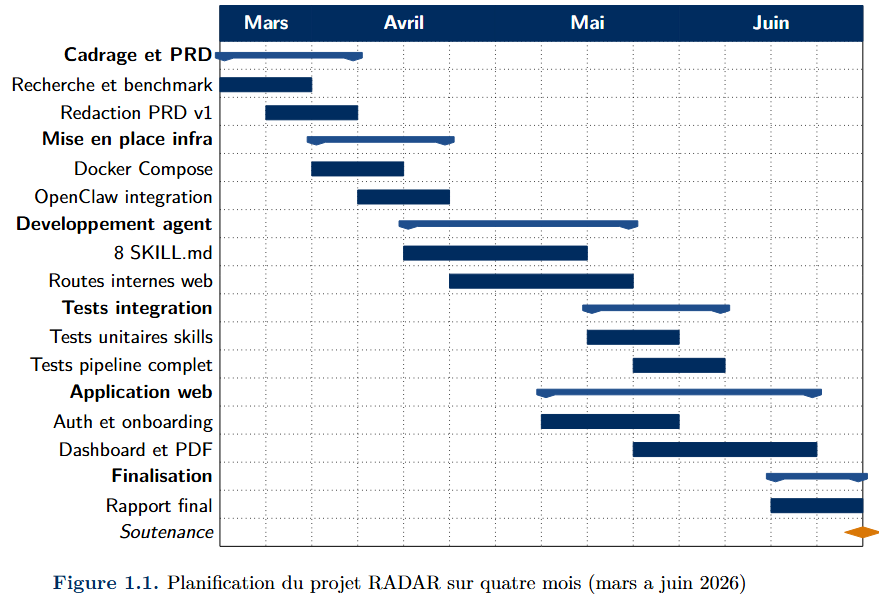
\includegraphics[width=\linewidth]{planification_radar.png}
  \caption{Diagramme de Gantt de la planification du projet RADAR}
  \label{fig:gantt-projet}
\end{figure}

\section{Cahier des charges simplifié}
\label{sec:cahier-charges}

RADAR n'est pas qu'un exercice scolaire : nous l'avons concu comme une offre que l'on pourrait facturer a un client. Le tableau \ref{tab:cahier-charges} formalise le cahier des charges de la version 1 dans cette logique de prestation.

\begin{table}[H]
  \centering
  \caption{Cahier des charges synthetique de RADAR V1}
  \label{tab:cahier-charges}
  \small
  \begin{tabularx}{\linewidth}{lY}
    \toprule
    \textbf{Rubrique} & \textbf{Engagement} \\
    \midrule
    Besoin client & Disposer chaque matin d'un rapport de veille concurrentielle structure, sans intervention manuelle, couvrant entre un et dix concurrents nommes par l'utilisateur. \\
    Fonctionnalites cles & Inscription guidee avec enrichissement automatique du profil entreprise (Deep Research), cycle de veille quotidien declenche par cron, dashboard temps reel, digest courrier electronique quotidien, export PDF. \\
    Contraintes techniques & Hebergement Docker mutualise ou self-hosted (VPS Hetzner CX21), dependance externe a DeepSeek (modele LLM) et Tavily (recherche web), reseau interne entre les services, persistance PostgreSQL. \\
    Indicateurs de succes & Rapport produit chaque jour avant 7h00, sources evaluees CRAAP avec score moyen superieur a 14 sur 20, recoupement minimum a deux sources independantes pour chaque alerte, taux d'echec inferieur a 5 pour cent par cycle. \\
    Delai de livraison & Une version operationnelle deployee sur VPS au plus tard une semaine avant la soutenance, c'est-a-dire mi-juin 2026. \\
    Ressources mobilisees & Deux developpeurs etudiants en cycle ingenieur, environ trente heures hebdomadaires chacun sur la duree du semestre. \\
    Resultats attendus & Une plateforme utilisable en mode demonstration pour le jury, un rapport documente, un depot Git public, et la capacite a soutenir une demonstration en direct sur un compte test. \\
    \bottomrule
  \end{tabularx}
\end{table}

Ce cahier des charges servira de reference tout au long du rapport : chaque choix technique presente dans les chapitres suivants pourra etre confronte aux engagements pris ici, et le chapitre 7 etablira un bilan honnete de ce qui a ete tenu et de ce qui reste a finaliser.

% =========================================================================
% CHAPITRE 2 - ETAT DE L'ART
% =========================================================================
\chapter{Etat de l'art}
\label{chap:etat-art}

Ce chapitre situe RADAR par rapport a deux univers qui le precedent : la veille strategique en tant que discipline, et l'ecosysteme des agents IA en tant que technologie. Il reste volontairement bref, l'objectif est de marquer et de fournir une compéhension plus large et de differencier notre solution du marché actuel.

\section{Concepts fondateurs de la veille strategique}
\label{sec:concepts-veille}

La veille strategique, discipline formalisee dans la litterature francophone par Humbert Lesca, est enseignee dans le module M244 du Pr. Younes Wadiai a travers quatre concepts que nous avons transposes directement dans le moteur RADAR.

Le \textbf{cycle de veille} en cinq etapes (identification des besoins, collecte, analyse et traitement, diffusion et exploitation, mise a jour continue) structure le pipeline de RADAR de bout en bout : chaque competence du moteur correspond a un segment du cycle.

L'evaluation des sources s'appuie sur la \textbf{grille CRAAP} (Currency, Relevance, Authority, Accuracy, Purpose), formalisee par Sarah Blakeslee en 2004. Chaque critere est note sur quatre points pour un score global sur vingt. La competence Evaluateur calcule ce score pour chaque source ; un seuil de cinq sur vingt declenche le filtrage.

L'analyse strategique mobilise les grilles \textbf{SWOT} (forces et faiblesses internes, opportunites et menaces externes) et \textbf{PESTEL} (six dimensions : politique, economique, sociologique, technologique, environnementale, legale). RADAR produit la SWOT quotidiennement et la PESTEL au rythme hebdomadaire.

Enfin, RADAR detecte les \textbf{signaux faibles} theorises par Igor Ansoff en 1975 dans \textit{Managing Strategic Surprise by Response to Weak Signals}. La competence dediee croise les sources mineures (forums, blogs, offres d'emploi) et majeures sur une fenetre glissante de trente jours stockee en base PostgreSQL, pour faire emerger des recurrences qui annoncent un mouvement de fond.

\section{Panorama des outils de veille existants}
\label{sec:panorama-outils}

Le marche de la veille concurrentielle est dense mais segmente. Les outils les plus connus repondent en realite a des besoins assez differents les uns des autres, et la plupart ne couvrent pas la veille strategique methodologique au sens du M244. Le tableau \ref{tab:benchmark-outils} dresse un panorama des solutions que nous avons examinees lors de la phase de cadrage.

\begin{table}[H]
  \centering
  \caption{Panorama compare des principaux outils de veille concurrentielle}
  \label{tab:benchmark-outils}
  \small
  \begin{tabularx}{\linewidth}{lYY}
    \toprule
    \textbf{Outil} & \textbf{Coeur metier} & \textbf{Limite par rapport a RADAR} \\
    \midrule
    Similarweb & Mesure du trafic web, classement par categorie, sources d'audience & Aucune analyse SWOT ni PESTEL, pas de detection de signaux faibles, oriente SEO et marketing \\
    SEMrush & Positionnement de mots-cles, backlinks, suivi de la presence digitale & Meme limite : centre sur le SEO, ne couvre pas la veille strategique \\
    Crayon & Veille concurrentielle enterprise avec battlecards et alerting & Tres oriente sales enablement grand compte, prix prohibitif pour une PME \\
    Mention & Social listening, mentions de marque, sentiment & Pas de cadre methodologique, ne produit pas de grille d'analyse \\
    Brandwatch & Social listening grand compte avec analytics avances & Meme remarque, plus la barriere du prix \\
    Google Alerts & Notification de nouveautes a partir de mots-cles & Beaucoup trop bruyant, aucune evaluation des sources, pas de structuration \\
    Feedly & Agregateur de flux RSS avec couche IA optionnelle & Centre sur la lecture, ne genere pas de synthese strategique \\
    \bottomrule
  \end{tabularx}
\end{table}

Aucun de ces outils ne fait du cycle M244 son fil conducteur. RADAR se positionne sur ce creneau libre : produire chaque jour des livrables strategiques structures par une methodologie explicite, a destination des PME et des consultants independants qui n'ont ni le budget ni le besoin des suites enterprise.

\section{Evolution des agents IA autonomes}
\label{sec:agents-ia}

Le terme \textit{agent} designe depuis longtemps en intelligence artificielle un programme capable de percevoir son environnement et d'agir pour atteindre un objectif. Le changement majeur intervient en 2023 avec l'arrivee des grands modeles de langage : le moteur de raisonnement n'est plus une suite de regles ecrites a la main, mais un LLM auquel on donne acces a des outils externes et a une memoire de travail. AutoGPT, publie en avril 2023, a popularise cette approche, suivi par des frameworks plus aboutis comme LangChain et son evolution LangGraph.

Les architectures actuelles reposent sur quatre briques : un LLM comme moteur de raisonnement, des outils pour agir au-dela du texte (recherche web, lecture de fichiers, execution de code), une memoire a court et long terme, et une boucle de controle qui decide quand mobiliser chaque outil.

OpenClaw, le runtime que nous avons retenu pour RADAR, integre ces briques dans un seul binaire compatible avec l'API OpenAI Chat Completions. Les comportements d'un agent se decrivent dans des fichiers Markdown \texttt{SKILL.md}, lisibles et modifiables sans recompilation. La fonction \texttt{sessions\_spawn} cree des sous-sessions isolees indispensables a un pipeline sequentiel, le cron natif gere le declenchement quotidien, et les outils \texttt{web\_search}, \texttt{web\_fetch} et \texttt{browser} sont disponibles sans configuration. Face a un paysage mouvant (Claude Agent SDK, Mastra, LangGraph, plateformes hebergees), notre choix repose sur le caractere open source du code, la compatibilite native avec l'API OpenAI qui ouvre la porte a tous les modeles disponibles dans cette interface, et la lisibilite immediate du format SKILL.md.

\section{Positionnement de RADAR}
\label{sec:positionnement-radar}

RADAR n'a pas vocation a remplacer Similarweb, ni a jouer le role d'un agregateur de flux, d'un social listener ou d'un framework d'agents generaliste. Sa specialite tient en une formule : automatiser le cycle de veille M244 pour des PME et des consultants, en transformant chaque concept du cours en une fonctionnalite produit observable.

Cette specialisation est a la fois la force et la limite du projet. Force, parce qu'elle assure une coherence methodologique que les outils generalistes n'ont pas : chaque source collectee est evaluee par CRAAP, chaque alerte est recoupee, chaque rapport suit la structure attendue par le cours. Limite, parce qu'elle restreint le perimetre fonctionnel et nous oblige a laisser de cote des sujets adjacents comme la veille brevet, la veille reglementaire ou la surveillance de la reputation en ligne. Ces sujets pourraient faire l'objet d'extensions, dont nous discutons dans les perspectives du chapitre 7.

% =========================================================================
% CHAPITRE 3 - ARCHITECTURE DE RADAR
% =========================================================================
\chapter{Architecture de RADAR}
\label{chap:architecture}

Ce chapitre presente l'architecture technique de RADAR : la maniere dont les composants s'articulent, les decisions structurantes qui ont oriente la conception, la stack retenue et les precautions prises pour l'isolation des sessions utilisateur.

\section{Schema global du systeme}
\label{sec:schema-global}

RADAR fonctionne sur trois services Docker independants qui collaborent via un reseau interne. Le premier est l'application web batie sur Next.js qui sert d'interface utilisateur et de couche de persistance. Le deuxieme est le moteur agent OpenClaw qui execute les huit competences specialisees. Le troisieme est la base de donnees PostgreSQL qui stocke profils, sources, analyses et rapports. La figure \ref{fig:archi-globale} schematise cette topologie.

\begin{figure}[H]
  \centering
  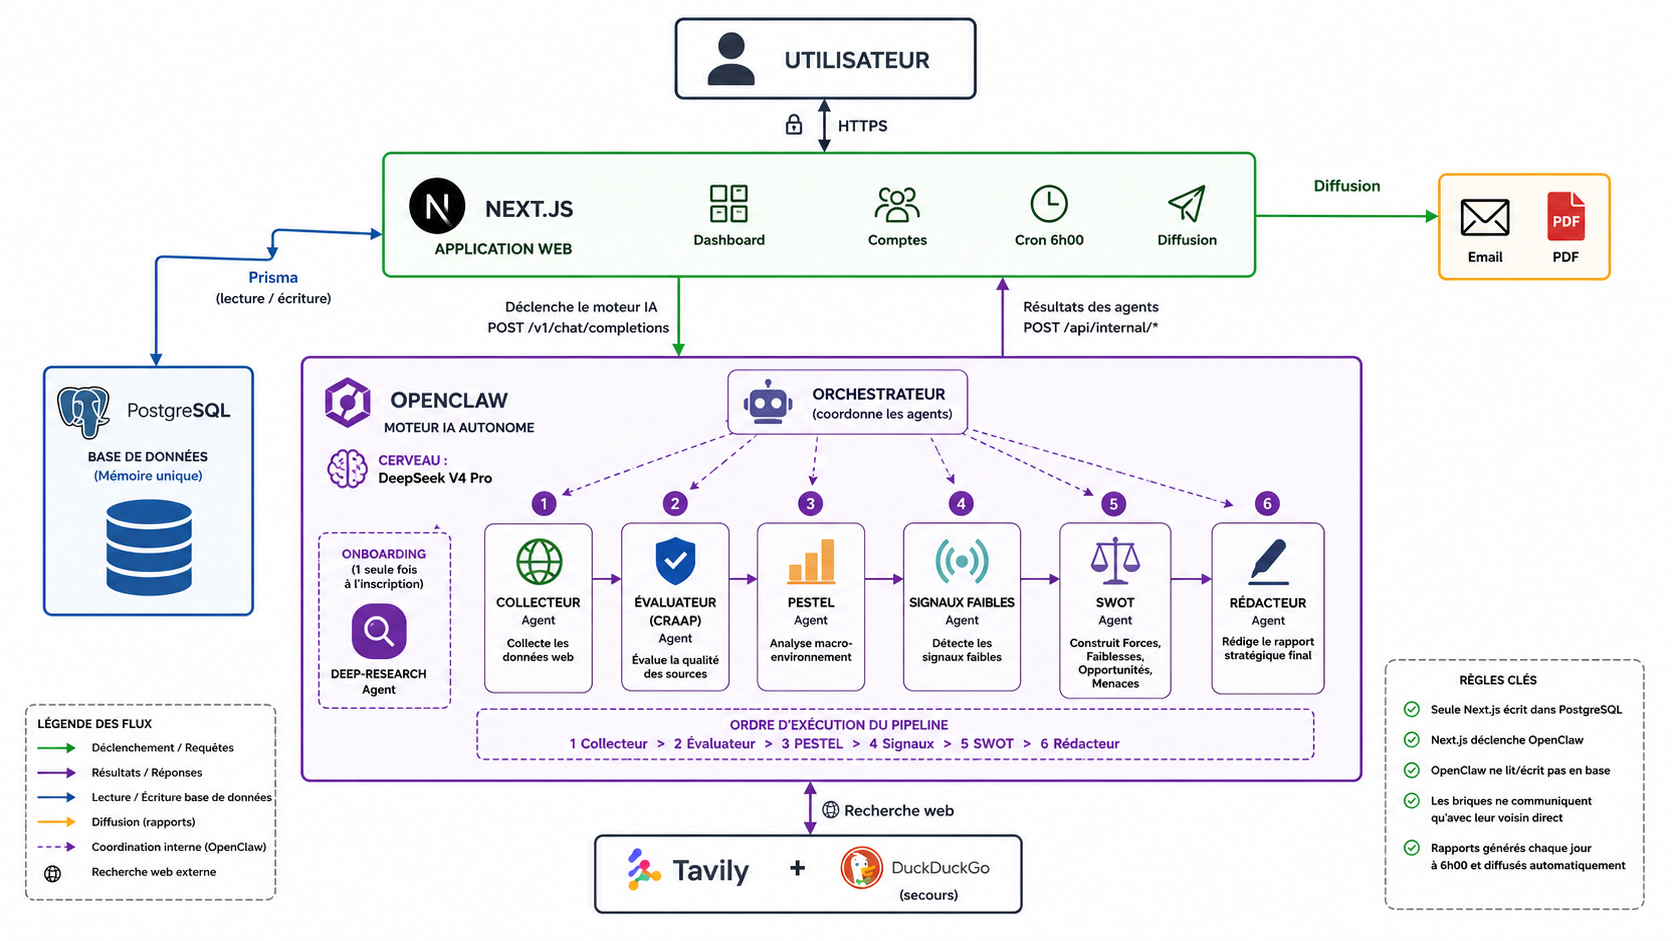
\includegraphics[width=\linewidth]{schema_global_radar.png}
  \caption{Architecture globale de RADAR}
  \label{fig:archi-globale}
\end{figure}

Le flux nominal d'un cycle de veille suit toujours la meme sequence. Un cron declenche l'orchestrateur a six heures du matin, ou un bouton dans le dashboard utilisateur peut le declencher a la demande. L'orchestrateur lit le profil utilisateur passe en parametre du message initial, puis enchaine les sous-sessions via \texttt{sessions\_spawn}. Chaque sous-session execute une competence : collecte, evaluation, analyses, detection des signaux faibles, redaction. Apres chaque etape, la competence envoie ses resultats a l'application web via une route interne dediee, et retourne son livrable a l'orchestrateur pour alimenter l'etape suivante. Une fois le cycle termine, le rapport final est marque comme acheve dans la base, et l'application web notifie l'utilisateur par courrier electronique.

\section{Choix d'architecture cles}
\label{sec:choix-architecture}

Cinq decisions structurantes ont oriente la conception. Nous les listons ici parce qu'elles conditionnent tous les chapitres suivants.

\begin{decisionBox}[title={Decision 1 : un seul agent OpenClaw avec huit competences, et non huit agents distincts}]
OpenClaw permet de definir plusieurs agents dans un meme processus. Chaque agent dispose alors de son propre modele, de ses propres outils, de sa propre memoire. Cette approche multi-agent a un cout : la communication entre agents passe par des messages externes, ce qui complique l'orchestration et augmente la latence. Nous avons prefere une architecture simple : un seul agent (l'agent \texttt{main}) qui charge huit competences au format SKILL.md. L'orchestration interne se fait alors via \texttt{sessions\_spawn}, qui cree des sous-sessions isolees du meme agent. Cette decision a ete validee apres lecture de la documentation OpenClaw : \texttt{sessions\_spawn} ne sait pas cibler un autre agent, il opere sur l'agent courant.
\end{decisionBox}

\begin{decisionBox}[title={Decision 2 : communication agent vers web via HTTP interne, sans signature HMAC}]
Les architectures de webhook classiques exigent une signature HMAC pour authentifier l'expediteur. RADAR utilise un reseau Docker interne ferme : seuls les conteneurs declares dans le meme \texttt{docker-compose.yml} peuvent atteindre les routes \texttt{/api/internal/*}. Cette isolation reseau rend la signature HMAC superflue en V1. Si le produit devait passer en multi-tenant heberge sans isolation reseau, l'ajout d'une couche HMAC serait la premiere chose a faire ; nous l'avons documente comme dette technique connue.
\end{decisionBox}

\begin{decisionBox}[title={Decision 3 : modele LLM DeepSeek V4 Pro, et non GPT-4o ni Claude Opus}]
Notre premier prototype utilisait GPT-4o. Il atteignait rapidement la limite de trente mille tokens par minute du Tier 1 OpenAI, ce qui bloquait la competence Deep Research qui consomme a elle seule pres de trente mille tokens sur le dernier appel. DeepSeek V4 Pro offre un contexte d'un million de tokens, une limite de debit elastique et un cout dix-sept fois inferieur a celui de GPT-4o, tout en restant compatible avec l'API OpenAI Chat Completions qu'OpenClaw exploite. La degradation de qualite par rapport a Claude Opus 4.7 sur les analyses SWOT et PESTEL est restee acceptable lors des tests d'integration.
\end{decisionBox}

\begin{decisionBox}[title={Decision 4 : Tavily comme provider primaire de recherche web, DuckDuckGo en fallback}]
DuckDuckGo est gratuit et fonctionne sans cle API, ce qui en a fait notre premier choix. Mais le moteur applique une detection de bot agressive sur les rafales de requetes, et la competence Collecteur en emet typiquement quinze a vingt par cycle. Tavily, concu pour les agents IA, retourne le contenu complet des pages (pas seulement les URL), n'applique pas de detection de rafales sur le free tier et offre mille requetes par mois. La competence Deep Research peut continuer a utiliser DuckDuckGo car ses requetes sont espacees dans le temps, mais le Collecteur passe par Tavily.
\end{decisionBox}

\begin{decisionBox}[title=Decision 5 : cron OpenClaw natif et orchestrateur sans persistance propre]
OpenClaw embarque un scheduler cron natif qui declenche un message initial vers un agent a l'heure configuree. Plutot que d'ajouter une couche de scheduling externe comme pg-boss ou node-cron du cote Next.js, nous nous sommes contentes du cron OpenClaw. L'orchestrateur lui-meme ne maintient pas d'etat persistant : chaque cycle est independant et l'integralite de la traçabilite remonte dans la base PostgreSQL via les routes internes. Cette simplicite reduit le nombre de composants a operer en production.
\end{decisionBox}

\section{Stack technique justifiee}
\label{sec:stack-technique}

Le tableau \ref{tab:stack} resume la stack technique retenue et les raisons de chaque choix.

\begin{table}[H]
  \centering
  \caption{Stack technique de RADAR et justification de chaque brique}
  \label{tab:stack}
  \small
  \begin{tabularx}{\linewidth}{lYY}
    \toprule
    \textbf{Couche} & \textbf{Technologie} & \textbf{Raison du choix} \\
    \midrule
    Frontend & Next.js 16, React 19, Tailwind CSS 4 & Standard de l'ecosysteme JavaScript, support natif du SSR et des Server Actions, communaute large \\
    Authentification & Better-Auth & Support Next.js App Router, OAuth Google integre, sessions DB-backed \\
    Base de donnees & PostgreSQL 17 & Robustesse, support JSONB pour les structures semi-structurees des analyses, gratuit \\
    ORM & Prisma 6 & Generation de types TypeScript a partir du schema, migrations versionnees \\
    Runtime Node & Node 24 & Derniere LTS au moment du projet, performances ameliorees \\
    Monorepo & pnpm 10, Turborepo & Gestion partagee des dependances, cache de build entre packages \\
    Moteur agent & OpenClaw (image \texttt{ghcr.io/openclaw/openclaw:latest}) & Open source, format SKILL.md lisible, sessions\_spawn natif \\
    Modele LLM & DeepSeek V4 Pro (\texttt{deepseek/deepseek-v4-pro}) & Contexte 1M tokens, cout dix-sept fois inferieur a GPT-4o, compatible API OpenAI \\
    Recherche web & Tavily (primaire), DuckDuckGo (fallback) & Tavily concu pour agents IA, pas de bot detection, contenu complet retourne \\
    Conteneurisation & Docker, Docker Compose & Standard d'industrie, environnement reproductible local et production \\
    Hebergement V1 & Hetzner Cloud CX21 & Cout maitrise (~4 EUR par mois), serveurs allemands conformes RGPD \\
    Envoi courriel & Resend & API simple, free tier suffisant pour V1, support DKIM \\
    \bottomrule
  \end{tabularx}
\end{table}

Cette stack a ete choisie pour optimiser deux variables a la fois : le cout d'exploitation, parce que le projet n'a aucun budget commercial, et la maintenabilite, parce qu'il doit pouvoir etre repris par un developpeur exterieur a l'equipe initiale. Chaque brique est mature, documentee et largement utilisee dans la communaute.

\section{Securite et isolation des sessions utilisateur}
\label{sec:securite}

La securite d'une plateforme qui agrege des donnees concurrentielles pour le compte de plusieurs clients meriterait un chapitre complet. Malgré que Radar est un MVP, mais plusieurs precautions ont ete prises des la conception pour eviter de creer une dette de securite difficile a rattraper.

\textbf{Isolation reseau.} Les trois services Docker (Next.js, OpenClaw, PostgreSQL) communiquent uniquement sur un reseau prive declare dans le \texttt{docker-compose.yml}. Seuls les ports HTTPS de l'application web sont exposes vers l'exterieur. OpenClaw n'est jamais accessible depuis Internet, ce qui ferme la plus grande surface d'attaque potentielle.

\textbf{Isolation des contextes utilisateur.} Chaque cycle de veille declenche une session OpenClaw dediee, dont le contexte se limite au profil utilisateur transmis dans le message initial. Le mecanisme \texttt{sessions\_spawn} cree des sous-sessions isolees pour chaque competence du pipeline, ce qui empeche la fuite de donnees entre etapes. Aucune memoire partagee entre utilisateurs n'est conservee cote agent ; toute la persistance passe par la base PostgreSQL ou les enregistrements sont strictement rattaches a leur \texttt{userId}.

\textbf{Secrets et cles API.} Toutes les cles externes (DEEPSEEK\_API\_KEY, TAVILY\_API\_KEY, OPENCLAW\_INTERNAL\_SECRET) sont passees aux conteneurs via des variables d'environnement, jamais commitees dans le depot Git. Le fichier \texttt{.env.example} documente la liste attendue sans contenir les valeurs reelles. Un fichier \texttt{.env} est requis localement et sur le VPS, place hors arborescence Git.

\textbf{Persistance des donnees.} La base PostgreSQL applique les bonnes pratiques standard : un utilisateur applicatif aux droits limites, des sauvegardes journalieres planifiees sur le VPS, des migrations versionnees via Prisma qui interdisent les modifications de schema manuelles en production.

\textbf{Authentification utilisateur.} Cote application web, Better-Auth gere les sessions DB-backed avec un identifiant opaque rotated regulierement, et le mot de passe est hashe avec Argon2id. Le detail de cette implementation est documente dans le chapitre 5.

Ces precautions constituent un socle defensif raisonnable pour un MVP. Le chapitre 7 detaille les renforcements de securite a prevoir en V2, notamment l'ajout d'une couche HMAC sur les routes internes, d'une politique de retention RGPD formalisee et d'un audit de dependances automatise.

% =========================================================================
% CHAPITRE 4 - IMPLEMENTATION DU MOTEUR AGENT
% =========================================================================
\chapter{Implementation du moteur agent}
\label{chap:moteur-agent}

Ce chapitre detaille la realisation du moteur agent de RADAR, c'est-a-dire la partie du systeme qui orchestre la collecte, l'evaluation, l'analyse et la redaction des rapports. Le moteur agent est entierement contenu dans le repertoire \texttt{apps/agent} du monorepo et se deploie comme un conteneur Docker autonome, accessible depuis l'application web via un reseau prive.

\section{Infrastructure Docker}
\label{sec:infra-docker}

Le moteur agent est livre sous la forme d'un service Docker dans le fichier \texttt{infra/docker/stack-complet/docker-compose.yml}. Trois services coexistent dans la stack : le service \texttt{postgres} (PostgreSQL 17), le service \texttt{openclaw} (image officielle \texttt{ghcr.io/openclaw/openclaw:latest}) et le service \texttt{web} qui porte l'application Next.js. Les trois services partagent un reseau Docker interne nomme \texttt{radar-net}, ce qui leur permet de communiquer par leur nom de service sans passer par l'exterieur.

Le service OpenClaw expose le port 18789, mais seulement vers le reseau interne. Les variables d'environnement DEEPSEEK\_API\_KEY, TAVILY\_API\_KEY et OPENCLAW\_INTERNAL\_SECRET sont passees au conteneur depuis le fichier \texttt{.env} place a la racine du projet. Le volume \texttt{apps/agent/openclaw-data} est monte dans le conteneur a l'emplacement \texttt{/data}, ce qui permet a OpenClaw d'y trouver sa configuration (\texttt{openclaw.json}), ses profils d'authentification (\texttt{auth-profiles.json}) et les fichiers SKILL.md des huit competences. Le volume \texttt{apps/agent/workspace} est monte de la meme maniere pour rendre l'arborescence des skills modifiable sans rebuild du conteneur.

La commande de demarrage typique depuis le dossier de la stack est la suivante :

\begin{lstlisting}[language=bash,caption={Commande de demarrage de la stack de developpement}]
cd infra/docker/stack-complet
docker compose --env-file "../../../.env" up -d
\end{lstlisting}


\section{Configuration OpenClaw}
\label{sec:config-openclaw}

Toute la configuration d'OpenClaw tient dans deux fichiers situes dans \texttt{apps/agent/openclaw-data}. Le premier, \texttt{openclaw.json}, decrit la structure du moteur : agents declares, modeles disponibles, providers de recherche web, parametres de scheduling et timeouts par defaut. Le second, \texttt{auth-profiles.json}, declare les profils d'authentification aupres des fournisseurs externes en mappant des cles symboliques sur les variables d'environnement.

Le fichier \texttt{openclaw.json} declare un seul agent nomme \texttt{main}. Cet agent charge tous les skills du dossier \texttt{workspace/skills}. Les parametres globaux retiennent une attention particuliere : \texttt{thinkingDefault} est positionne a \texttt{medium}, ce qui active le raisonnement intermediaire de DeepSeek V4 Pro sans le pousser a son maximum (le mode \texttt{xhigh} multipliait par trois la duree des cycles pour un gain de qualite marginal sur nos tests). Le parametre \texttt{timeoutSeconds} est fixe a 900 (quinze minutes), ce qui couvre largement la duree typique d'une competence du pipeline. Le scheduling est configure pour declencher l'agent \texttt{main} tous les jours a six heures du matin, fuseau \texttt{Africa/Casablanca}, mais en pratique nous laissons ce declencheur cote application web pour faciliter la gestion multi-utilisateur.

L'extrait suivant illustre les blocs essentiels de \texttt{openclaw.json} :

\begin{lstlisting}[language={},caption={Extrait significatif de openclaw.json}]
{
  "agents": {
    "defaults": {
      "model": "deepseek/deepseek-v4-pro",
      "thinkingDefault": "medium",
      "timeoutSeconds": 900,
      "fastDefault": "off"
    },
    "list": [
      { "id": "main", "skillsDir": "workspace/skills" }
    ]
  },
  "plugins": {
    "tavily": { "apiKeyEnv": "TAVILY_API_KEY" },
    "duckduckgo": { "enabled": true }
  },
  "scheduler": {
    "crons": [
      { "agent": "main", "expr": "0 6 * * *", "tz": "Africa/Casablanca" }
    ]
  }
}
\end{lstlisting}

\section{Architecture skills versus agents}
\label{sec:skills-vs-agents}

\begin{figure}[H]
  \centering
  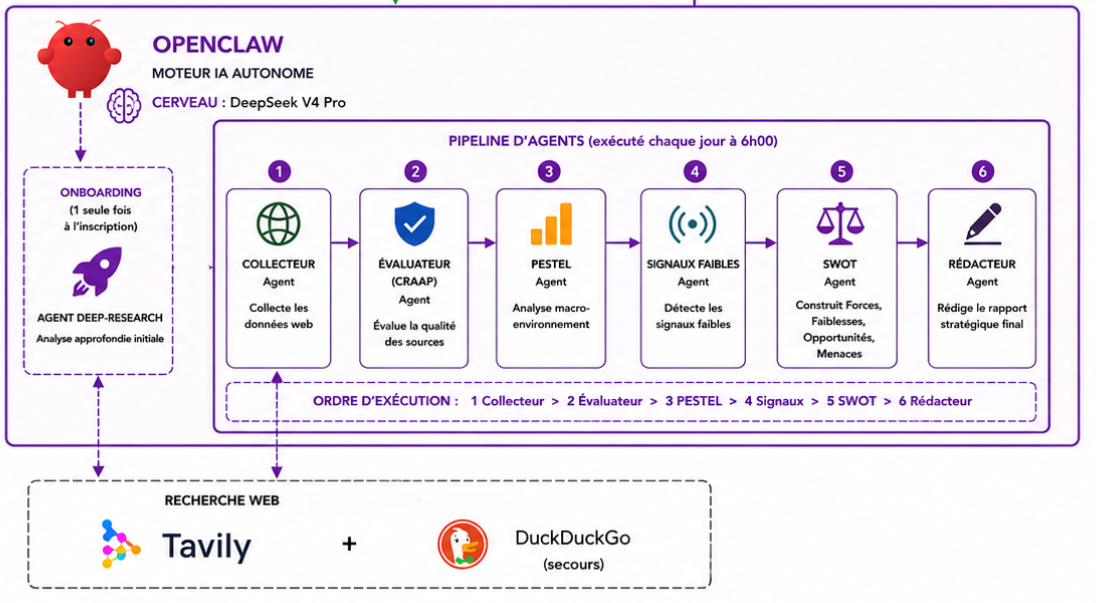
\includegraphics[width=\linewidth]{Config_agent.png}
  \caption{Configuration retenue : un agent chargeant huit competences}
  \label{fig:config-agent}
\end{figure}

Cette section explique la decision la plus structurante du projet : un seul agent qui charge huit competences, plutot que huit agents distincts.

Dans OpenClaw, un agent est une entite complete avec son modele LLM, ses outils et sa memoire. Une competence (skill) est plus legere : un script de comportement decrit dans un fichier \texttt{SKILL.md} compose d'un en-tete YAML et d'un corps en Markdown libre. Le mode multi-agent d'OpenClaw permet de faire cohabiter plusieurs agents dans un meme processus, mais il est concu pour router des messages externes vers le bon agent, pas pour orchestrer un pipeline interne : la communication inter-agents passerait par des allers-retours HTTP couteux qui dilueraient le contexte.

La fonction \texttt{sessions\_spawn} repond exactement a notre besoin. Elle cree une sous-session du meme agent avec un contexte vierge, ce qui correspond a la logique d'un pipeline sequentiel ou chaque etape doit demarrer proprement avant d'alimenter la suivante.

Une derniere contrainte a tranche le debat : le YAML de \texttt{SKILL.md} ne permet pas de surclasser le modele LLM ni le niveau de \texttt{thinking} par competence. Apres tests, un \texttt{thinking=medium} global s'est revele satisfaisant pour toutes les etapes, ce qui retire l'unique raison qui nous aurait pousses vers le multi-agent.

\section{Les huit competences SKILL.md}
\label{sec:huit-skills}

Le pipeline de RADAR repose sur huit competences specialisees. Cette section presente chacune d'elles, son role dans le cycle, ses entrees et ses sorties.

\subsection{Deep Research}
\label{sec:skill-deep-research}

Deep Research est la seule competence du moteur qui s'execute en dehors du pipeline orchestre. Elle est declenchee une seule fois par utilisateur, au moment de l'inscription, et ne participe a aucun cycle de veille quotidien. Son execution est independante : elle n'est pas appelee par l'orchestrateur et n'alimente pas directement les sept autres competences dans la meme session ; son resultat est stocke en base pour que les cycles ulterieurs puissent le reutiliser.

Son role est de transformer un couple basique \og nom d'entreprise + site web \fg{} en un profil enrichi exploitable par le reste du systeme : secteur d'activite, taille (\texttt{sizeBand}), ville du siege, produits principaux, clientele cible (\texttt{ICP}), positionnement, mots-cles metier et concurrents potentiellement non listes par l'utilisateur.

Deep Research utilise les outils natifs d'OpenClaw \texttt{web\_search} et \texttt{web\_fetch}. Sur DuckDuckGo plutot que sur Tavily, parce que ses requetes sont espacees dans le temps (typiquement trois ou quatre requetes sur cinq minutes) et qu'elle ne declenche donc pas la detection de bot. Le SKILL.md decrit une procedure en quatre temps : recherche du site officiel, recherche d'informations annexes (presse, LinkedIn, registres d'entreprise), recoupement, et synthese au format JSON attendu.

La sortie de Deep Research est postee directement sur \texttt{/api/internal/profil} avec la structure \texttt{ProfilUtilisateur}. Le profil reste \emph{permanent} en base : il sera lu a chaque cycle de veille et passe a l'orchestrateur dans le message initial. La motivation de cette decision est economique : Deep Research consomme environ trente mille tokens DeepSeek, et il serait absurde de relancer cette consommation a chaque cycle alors que le profil d'une entreprise change peu sur des semaines.

\subsection{Orchestrateur}
\label{sec:skill-orchestrateur}

L'orchestrateur est le chef d'orchestre du pipeline quotidien. Il n'execute aucune tache propre : il enchaine les sous-sessions via \texttt{sessions\_spawn} et propage les resultats d'une etape a l'autre. Il est declenche soit par le cron OpenClaw a six heures, soit par un appel HTTP venant de l'application web (bouton \og Lancer un cycle maintenant \fg{} dans le dashboard).

L'entree de l'orchestrateur est un message qui contient l'identifiant du rapport (\texttt{rapportId}), l'identifiant utilisateur (\texttt{userId}), le profil complet de l'entreprise utilisatrice (deja produit par Deep Research et stocke en base) et la liste des concurrents a surveiller. Cette charge utile est suffisamment volumineuse pour que nous ayons documente sa structure dans le SKILL.md de l'orchestrateur, afin que les autres competences sachent exactement ce qu'elles peuvent attendre lorsqu'elles sont invoquees.

La sortie principale de l'orchestrateur est un POST vers \texttt{/api/internal/rapport/termine} contenant le rapport final. En parallele, apres chaque etape, l'orchestrateur POST vers \texttt{/api/internal/rapport/progresse} pour notifier l'application web de l'avancement. En cas d'erreur (timeout, exception, retour incoherent d'une competence), il POST vers \texttt{/api/internal/rapport/echec} avec le motif. Cette triple route permet a l'utilisateur de suivre la progression en temps reel dans son dashboard.

Une particularite importante decouverte lors des tests : la valeur de \texttt{runTimeoutSeconds} passee a chaque appel de \texttt{sessions\_spawn} ecrase le \texttt{timeoutSeconds} global de la configuration OpenClaw. Le SKILL.md de l'orchestrateur fixe explicitement ce parametre a 900 secondes pour chaque etape, sinon la valeur par defaut de 300 secondes s'appliquait et faisait echouer l'evaluateur ou les analystes sur les rapports denses.

\subsection{Collecteur}
\label{sec:skill-collecteur}

Le collecteur est la premiere etape executive du pipeline quotidien. Il recoit en entree le profil utilisateur et la liste des concurrents, et il doit produire un ensemble de sources fraiches couvrant les mouvements strategiques des concurrents sur les trois derniers jours.

La logique du collecteur est decrite en quatre phases dans son SKILL.md. La phase 1 etablit la liste des cibles a interroger : pour chaque concurrent, le site officiel cite explicitement dans le profil constitue une source primaire directe. La phase 2 invoque \texttt{web\_search} avec Tavily, en formant pour chaque concurrent des requetes ciblees sur les axes activees par l'utilisateur (recrutements, strategie, technologie, presence digitale, conformite). La phase 3 collecte les URL retournees et leur contenu (Tavily renvoie le contenu complet des pages dans la reponse de l'API, pas seulement les liens). La phase 4 applique un filtrage temporel strict : toute source dont la date connue est anterieure a la fenetre des trois derniers jours est ecartee, sans exception de pertinence.

Le SKILL.md inclut une logique conditionnelle pour gerer le fallback. Si la cle \texttt{TAVILY\_API\_KEY} est presente dans l'environnement, le collecteur passe par Tavily. Si elle est absente, il bascule sur DuckDuckGo en limitant la cadence a trois requetes maximum par batch et en effectuant \texttt{web\_fetch} pour recuperer le contenu des pages (DuckDuckGo ne retourne que des URL). Cette logique conditionnelle a evite plusieurs heures de bot blocking lors des premieres semaines de developpement, avant que nous ne prenions une cle Tavily.

La sortie du collecteur est une liste JSON de sources, chaque source contenant URL, titre, date detectee, extrait textuel et concurrent associe. Cette liste est POSTee vers \texttt{/api/internal/sources} pour persistance, et retournee a l'orchestrateur dans un bloc \texttt{json} explicite, ce qui permet a l'orchestrateur de la transmettre directement a l'evaluateur sans la reconstruire.

\subsection{Evaluateur}
\label{sec:skill-evaluateur}

L'evaluateur recoit la liste des sources collectees et calcule pour chacune un score CRAAP detaille. Les cinq criteres (Currency, Relevance, Authority, Accuracy, Purpose) sont notes sur quatre points chacun, ce qui donne un score global sur vingt. Une source dont le score global descend en dessous de cinq sur vingt est marquee \texttt{rejetee=true} et n'alimente pas les analyses en aval.

Le traitement des sources se fait par lots de cinq pour eviter les timeouts. Cette decision est venue apres un premier test ou l'evaluateur tentait de scorer dix-neuf sources en un seul appel, ce qui dependait massivement de la latence DeepSeek et finissait par excéder le timeout. Le batch de cinq combine a un timeout de 900 secondes a stabilise le composant : les cycles de tests ulterieurs ont tous abouti avec un score CRAAP moyen entre 14 et 16 sur 20 sur des cas reels.

La sortie de l'evaluateur est un POST vers \texttt{/api/internal/sources} avec les sources enrichies des scores CRAAP detaille (chaque critere et le total), de la decision \texttt{rejetee} et d'une justification courte par source. Cette information est essentielle pour l'audit: un evaluateur peut reproduire le calcul a la main sur n'importe quelle source pour verifier la coherence.

\subsection{Analyste PESTEL}
\label{sec:skill-pestel}

L'analyste PESTEL analyse l'environnement sectoriel global plutot qu'une organisation specifique. Il segmente cet environnement en six dimensions (politique, economique, sociologique, technologique, environnementale, legale) et produit pour chacune un ensemble de facteurs influents.

Les entrees sont la liste des sources evaluees, filtrees par un seuil de score CRAAP superieur ou egal a six sur vingt et un score Currency superieur ou egal a deux sur quatre. Ce double filtre evite que des sources marginalement acceptables (CRAAP=6) mais tres anciennes (Currency=1) ne polluent l'analyse. Le SKILL.md demande explicitement de mentionner pour chaque facteur PESTEL la dimension concernee, l'intensite de l'impact (faible, moyenne, forte), le sens (positif, negatif, neutre) et un ou plusieurs identifiants de sources qui le justifient.

La sortie est postee vers \texttt{/api/internal/pestel}. La dimension est rappelee dans chaque entree, ce qui rend la structure auto-portante : meme isolee de son contexte, une analyse PESTEL produite par RADAR reste exploitable. Cette sortie alimente directement l'etape suivante du pipeline, l'analyste SWOT.

\subsection{Analyste SWOT}
\label{sec:skill-swot}

L'analyste SWOT produit une grille classique en quatre quadrants : forces internes, faiblesses internes, opportunites externes, menaces externes. La grille porte sur l'entreprise utilisatrice et non sur les concurrents pris individuellement, car le M244 enseigne la SWOT comme un outil d'analyse \emph{de l'organisation dans son environnement}, pas comme un benchmark concurrent par concurrent.

Les entrees de l'analyste sont le profil utilisateur enrichi (issu de Deep Research), la liste des sources evaluees (filtrees par CRAAP $\geq 6$ et Currency $\geq 2$) et surtout la grille PESTEL produite a l'etape precedente. La PESTEL alimente directement les deux quadrants externes de la SWOT : chaque facteur sectoriel identifie par l'analyste PESTEL est repris et reformule du point de vue specifique de l'entreprise utilisatrice, ce qui donne les opportunites et les menaces. Les forces et les faiblesses internes sont quant a elles deduites du profil utilisateur croise avec les sources collectees sur l'entreprise. Ce chainage garantit la coherence entre la lecture macro de l'environnement et l'analyse strategique propre a l'entreprise.

La sortie de l'analyste est un POST vers \texttt{/api/internal/swot} avec un objet JSON structure : une liste de forces, une liste de faiblesses, une liste d'opportunites, une liste de menaces, et un score de confiance global compris entre zero et un. Chaque element est accompagne d'une justification courte qui pointe vers les sources mobilisees.

\subsection{Detecteur de signaux faibles}
\label{sec:skill-signaux}

Cette competence est la plus exigeante methodologiquement. Elle ne cherche pas dans les sources les informations explicites, mais les indices precoces qui annoncent un mouvement de fond. Elle recoit en entree non seulement les sources du cycle courant, mais aussi les sources des trente derniers jours conservees en base.

Le SKILL.md demande au detecteur de raisonner sur des accumulations : un sujet qui revient sur plusieurs sources mineures (forums, blogs, offres d'emploi), une thematique qui prend de l'ampleur sans avoir fait l'objet d'annonces officielles, un faisceau d'indices convergents qui pointe vers une decision strategique a venir. Pour chaque signal detecte, il produit une intensite (faible, moyenne, forte), un horizon temporel d'occurrence (court, moyen, long terme), un libelle, une description et la liste des sources qui le supportent.

La sortie est postee vers \texttt{/api/internal/signaux}. Contrairement aux analyses SWOT et PESTEL qui filtrent strictement par score CRAAP, le detecteur conserve les sources de score moderement bas (3 a 5) parce que la veille des signaux faibles passe necessairement par des sources de qualite mixte. Le SKILL.md le mentionne explicitement pour eviter de reproduire le filtre des analystes.

\subsection{Redacteur}
\label{sec:skill-redacteur}

Le redacteur recoit en entree la totalite des sorties precedentes : profil utilisateur, sources evaluees, grille PESTEL, grille SWOT, liste de signaux faibles. Il produit un rapport narratif structure qui suit le plan academique enseigne dans le module M244 : synthese executive, methodologie et collecte, analyse, resultats, recommandations strategiques.

Le SKILL.md du redacteur impose une structure en six sections avec des contraintes de longueur indicatives : entre cent et cent cinquante mots pour la synthese executive, et entre mille et mille cinq cents mots pour le rapport complet. Le ton est neutre, factuel, pas commercial. La sortie inclut egalement cinq recommandations strategiques chiffrees (priorite, effort, impact attendu) et un score de confiance global sur le cycle.

Le redacteur ne POST pas son rapport vers une route specifique. Il retourne le rapport complet a l'orchestrateur qui se charge du POST vers \texttt{/api/internal/rapport/termine} pour cloturer le cycle. Cette delegation evite que le redacteur n'ait a connaitre les conventions de l'API interne et le maintient dans son role de \og generateur de texte \fg{}.

\section{Integration de DeepSeek V4 Pro}
\label{sec:integration-deepseek}

Le choix du modele LLM s'est fait Après les tests serieux: GPT-4o, était la référence pour un fonctionnement correcte donc tous les modèles équivalant où plus performent que GPT-4o sont admissible. Le tableau \ref{tab:comparatif-llm} resume les criteres qui ont conduit a retenir DeepSeek V4 Pro pour RADAR.

\begin{table}[H]
  \centering
  \caption{Comparatif des modeles LLM evalues pour RADAR}
  \label{tab:comparatif-llm}
  \small
  \begin{tabularx}{\linewidth}{lYYY}
    \toprule
    \textbf{Critere} & \textbf{GPT-4o} & \textbf{Claude Opus 4.7} & \textbf{DeepSeek V4 Pro} \\
    \midrule
    Contexte maximal & 128k tokens & 200k tokens & \textbf{1M tokens} \\
    Cout entree (par M tokens) & 5 \$ & 15 \$ & \textbf{0{,}30 \$} \\
    Cout sortie (par M tokens) & 15 \$ & 75 \$ & \textbf{1{,}20 \$} \\
    Limite de debit & 30k TPM (Tier 1) & moderee & \textbf{elastique} \\
    Qualite analyses SWOT/PESTEL & Bonne & \textbf{Excellente} & Tres bonne \\
    Compatibilite API OpenAI & Native & Non & \textbf{Native} \\
    Adapte au budget academique & Non & Non & \textbf{Oui} \\
    \bottomrule
  \end{tabularx}
\end{table}

GPT-4o a ete ecarte sur le couple debit/cout : sa limite de 30k tokens par minute au Tier 1 saturait des le premier appel de Deep Research (environ 28k tokens), et un cycle complet aurait coute pres d'un dollar, soit plusieurs centaines de dollars par mois pour quelques comptes de test. Claude Opus 4.7 produit des analyses qualitativement superieures, mais son tarif (quinze dollars par million de tokens d'entree) reste hors de portee d'une plateforme livree gratuitement. DeepSeek V4 Pro combine un contexte d'un million de tokens, un cout dix-sept fois inferieur a GPT-4o, une limite de debit elastique et une compatibilite native avec l'API OpenAI utilisee par OpenClaw. Son integration s'est limitee a un changement d'URL et de cle dans \texttt{auth-profiles.json}.

\section{Integration de Tavily et fallback DuckDuckGo}
\label{sec:integration-tavily}

Le moteur de recherche web est essentiel au collecteur : sans lui, RADAR n'a rien a evaluer. Nous avons d'abord teste DuckDuckGo, gratuit et sans cle API. Probleme : il bloque l'adresse IP des qu'on emet trop de requetes rapprochees, et le collecteur en envoie quinze a vingt en moins d'une minute, ce qui declenchait systematiquement le blocage.

Nous sommes donc passes a Tavily, un moteur de recherche concu pour les agents IA. Il offre mille requetes mensuelles gratuites, retourne directement le contenu complet des pages dans sa reponse JSON, et n'applique pas de limite de cadence. La consommation typique de RADAR (environ quarante requetes par cycle) reste largement dans cette enveloppe.

Le SKILL.md du collecteur gere le basculement automatiquement : si la cle \texttt{TAVILY\_API\_KEY} est presente, il utilise Tavily ; sinon il revient sur DuckDuckGo avec des requetes ralenties (batchs de trois) et un \texttt{web\_fetch} complementaire pour recuperer le contenu des pages. Deep Research, dont les requetes sont naturellement espacees, reste sur DuckDuckGo pour economiser le quota Tavily.

\section{Communication entre agent et application web}
\label{sec:communication-agent-web}

La communication entre le moteur agent et l'application web se fait integralement en HTTP, sur le reseau Docker interne. Chaque competence et l'orchestrateur lui-meme effectuent des POST vers des routes nommees \texttt{/api/internal/*} portees par l'application Next.js. Ces routes sont decrites en detail dans le chapitre 5.

Le tableau \ref{tab:routes-internes} synthetise les routes attendues et leur utilisation cote agent.

\begin{table}[H]
  \centering
  \caption{Routes internes consommees par le moteur agent}
  \label{tab:routes-internes}
  \small
  \begin{tabularx}{\linewidth}{lYY}
    \toprule
    \textbf{Route} & \textbf{Appelant} & \textbf{Charge utile principale} \\
    \midrule
    POST \texttt{/api/internal/profil} & Deep Research & Profil enrichi de l'entreprise utilisatrice \\
    POST \texttt{/api/internal/sources} & Collecteur (creation) puis Evaluateur (mise a jour CRAAP) & Liste des sources avec metadonnees et scores \\
    POST \texttt{/api/internal/pestel} & Analyste PESTEL & Grille PESTEL six dimensions avec intensite et sens \\
    POST \texttt{/api/internal/swot} & Analyste SWOT & Grille SWOT structuree avec score de confiance \\
    POST \texttt{/api/internal/signaux} & Detecteur & Liste des signaux faibles avec intensite et horizon \\
    POST \texttt{/api/internal/rapport/progresse} & Orchestrateur (apres chaque etape) & Avancement du cycle pour notification dashboard \\
    POST \texttt{/api/internal/rapport/termine} & Orchestrateur (fin de cycle) & Rapport final, recommandations, score global \\
    POST \texttt{/api/internal/rapport/echec} & Orchestrateur (en cas d'erreur) & Motif d'echec, etape concernee, contexte \\
    \bottomrule
  \end{tabularx}
\end{table}

Toutes les requetes sont en JSON. L'identifiant du rapport (\texttt{rapportId}) accompagne chaque appel pour assurer la coherence : c'est cet identifiant qui sert de cle de regroupement en base de donnees. La reponse attendue est un objet \texttt{\{ success: true \}} si tout s'est bien passe, ou un objet \texttt{\{ success: false, error: <message> \}} dans le cas contraire. Le SKILL.md de chaque competence interprete la reponse et leve une exception si \texttt{success} vaut \texttt{false}, ce qui propage l'erreur a l'orchestrateur.

L'envoi parallele d'un POST de persistance et le retour direct du resultat a l'orchestrateur (pour alimenter la prochaine etape du pipeline) constituent ce que nous appelons le \og principe hybride \fg{} dans la documentation interne. Il garantit a la fois la visibilite temps reel dans le dashboard et la fluidite du pipeline interne, sans dependre du delai de re-lecture en base.

\section{Gestion des timeouts et fiabilite du pipeline}
\label{sec:timeouts-fiabilite}

Un pipeline d'agents qui appelle des services externes pendant pres d'une heure ne tient pas sans strategie explicite de gestion des erreurs et des timeouts. Nous avons travaille sur plusieurs fronts.

Le batching cote evaluateur est la premiere precaution prise. Comme decrit en section \ref{sec:skill-evaluateur}, le scoring CRAAP est effectue par lots de cinq sources. Cette taille de lot resulte d'un compromis : trop petit, le nombre d'appels DeepSeek explose et la latence cumulee allonge le cycle ; trop grand, chaque appel risque le timeout. Cinq sources par lot s'est revele etre le point d'equilibre apres iterations.

La gestion fine des timeouts est venue plus tard, apres un debug couteux. Comme mentionne en section \ref{sec:skill-orchestrateur}, le parametre \texttt{runTimeoutSeconds} passe a chaque \texttt{sessions\_spawn} ecrase le \texttt{timeoutSeconds} global. Nous avons fixe ce parametre a 900 secondes (quinze minutes) pour chaque etape, ce qui couvre largement le pire cas observe (l'evaluateur sur dix-neuf sources, environ douze minutes). Le diagnostic de cette subtilite a coute deux cycles de test echoues avant d'etre identifie : sans cette consigne explicite, le timeout par defaut de 300 secondes faisait echouer systematiquement les etapes d'analyse les plus denses.

Reste la traçabilite des erreurs. Chaque exception levee dans une competence ou dans l'orchestrateur produit un POST vers \texttt{/api/internal/rapport/echec} avec un motif lisible, l'identifiant du rapport et l'etape concernee. Cote serveur, ce POST cree un enregistrement \texttt{EvenementRapport} de type \texttt{ECHEC} dans la table dediee. L'utilisateur voit alors dans son dashboard l'etat \og echoue \fg{} avec le motif, plutot qu'un cycle qui reste bloque en \og en cours \fg{} indefiniment.

Ces precautions cumulees ont stabilise le pipeline au point que les trois derniers cycles de test (rapport-test-005 inclus) se sont tous termines avec succes en moins d'une heure, sur des cas reels et avec un score CRAAP moyen superieur a 16 sur 20.

% =========================================================================
% CHAPITRE 5 - IMPLEMENTATION DE L'APPLICATION WEB (KARAMO)
% =========================================================================
\chapter{Implementation de l'application web}
\label{chap:application-web}

\begin{noteBox}[title=Note de l'editeur du rapport]
Ce chapitre documente la realisation de l'application web Next.js qui sert d'interface utilisateur, gere l'authentification, persiste les donnees via Prisma et orchestre la livraison des rapports finaux. Le contenu detaille des sections ci-dessous est en cours de finalisation au moment de cette version du rapport.
\end{noteBox}

\section{Stack Next.js 16, React 19 et Tailwind CSS}
\label{sec:karamo-stack}

% À compléter

\section{Authentification et gestion utilisateur}
\label{sec:karamo-auth}

% À compléter

\section{Onboarding et tableau de bord}
\label{sec:karamo-dashboard}

% À compléter

\section{Routes API internes}
\label{sec:karamo-api}

% À compléter

\section{Modele de donnees Prisma et PostgreSQL}
\label{sec:karamo-prisma}

% À compléter

\section{Generation PDF et envoi par courrier electronique}
\label{sec:karamo-pdf-email}

% À compléter

% =========================================================================
% CHAPITRE 6 - TESTS ET VALIDATION DU SYSTEME
% =========================================================================
\chapter{Tests et validation du systeme}
\label{chap:tests}

Ce chapitre rend compte de la demarche de tests menee pendant le projet.

\section{Tests unitaires}
\label{sec:tests-unitaires}

Les tests unitaires valident le moteur agent en mode isole, sans dependance vis-a-vis de l'application web. Ils reposent sur la stack Docker du moteur dans laquelle le mock-api Node.js remplace l'application web : il expose les huit routes \texttt{/api/internal/*} et persiste chaque appel recu dans \texttt{apps/agent/openclaw-data/tests/}, sous un sous-dossier dedie a la competence appelante. Les fichiers sont horodates au format ISO, ce qui permet de reconstituer le deroule chronologique d'un cycle complet a partir des seules archives. Le dispositif est reproductible et auditable : un evaluateur exterieur peut relancer un cycle et comparer les fichiers produits a ceux versionnes dans le depot.

\subsection{Cas Marjane : test isole de Deep Research}
\label{sec:test-marjane}

Le premier test a porte sur la competence Deep Research, executee seule sur le cas Marjane, distributeur generaliste marocain choisi pour la richesse et l'heterogeneite de sa presence en ligne. La competence a produit en environ quatre minutes un profil de huit kilooctets de JSON contenant : le secteur (distribution generaliste), la taille (plus de 5000 employes), le siege (Casablanca), une liste de douze enseignes ou produits principaux, un descriptif de la clientele cible, un positionnement strategique, quinze mots-cles metier et cinq concurrents probables. L'execution s'est faite via DuckDuckGo, sans declencher de detection de bot.

\subsection{Cycle complet : rapport-test-005}
\label{sec:test-005}

Le test du cycle complet, identifie \texttt{rapport-test-005}, a ete execute le 7 mai 2026 entre 22h59 et 23h45. Il s'agit du premier cycle propre avec Tavily comme provider primaire. Les resultats sont resumes dans le tableau \ref{tab:resultats-test-005}.

\begin{table}[H]
  \centering
  \caption{Resultats du cycle de test rapport-test-005 (mai 2026)}
  \label{tab:resultats-test-005}
  \small
  \begin{tabularx}{\linewidth}{lY}
    \toprule
    \textbf{Metrique} & \textbf{Valeur observee} \\
    \midrule
    Provider de recherche utilise & Tavily (cle dans \texttt{TAVILY\_API\_KEY}) \\
    Nombre de sources collectees & 20 \\
    Score CRAAP moyen apres evaluation & 16{,}15 / 20 \\
    Nombre de sources rejetees (CRAAP < 5) & 0 \\
    Facteurs PESTEL identifies & 21 (repartis sur les 6 dimensions) \\
    Forces SWOT identifiees & 6 \\
    Faiblesses SWOT identifiees & 5 \\
    Opportunites SWOT identifiees & 6 \\
    Menaces SWOT identifiees & 6 \\
    Signaux faibles detectes & 8 (3 intensite forte, 4 moyenne, 1 faible) \\
    Recommandations strategiques produites & 5 \\
    Score de confiance global & 0{,}82 \\
    Duree totale du cycle & 46 minutes \\
    Taille du rapport narratif final & ~1400 mots structures en 6 sections \\
    \bottomrule
  \end{tabularx}
\end{table}

Tous les POST attendus vers les routes internes ont retourne \texttt{\{success: true\}}. Le rapport final, archive dans \texttt{tests/orchestrateur/termine-2026-05-07T23-45.json}, respecte la structure du cycle M244 et propose des recommandations chiffrees et priorisees.

\subsection{Echecs rencontres et corrections}
\label{sec:tests-echecs}

Deux cycles ont echoue avant le succes de \texttt{rapport-test-005}, et leurs causes ont nourri directement les corrections du moteur.

\textbf{rapport-test-003.} L'evaluateur a depasse le timeout de 300 secondes en tentant de scorer dix-neuf sources d'un coup, et le collecteur n'avait pas retourne sa liste dans un bloc JSON exploitable. Corrections appliquees : batching par lots de cinq sources cote evaluateur, et exigence explicite de \og Reponse finale OBLIGATOIRE avec bloc \texttt{```json}\fg{} dans le SKILL.md du collecteur.

\textbf{rapport-test-004.} L'evaluateur a fonctionne correctement, mais l'analyste PESTEL a depasse le timeout. Le diagnostic a revele que le \texttt{runTimeoutSeconds} par defaut (300 secondes) ecrasait silencieusement le \texttt{timeoutSeconds=900} global lorsqu'il n'etait pas declare explicitement dans chaque appel \texttt{sessions\_spawn}. Correction : fixation a 900 secondes dans tous les appels \texttt{sessions\_spawn} de l'orchestrateur.

Ces echecs ont egalement revele que DeepSeek conserve le contexte d'une conversation precedente dans la meme session OpenClaw, ce qui faisait remonter d'anciennes sources DuckDuckGo dans des tests Tavily. Le protocole de test a donc ete ajuste : nouvelle conversation a chaque lancement, et nettoyage de \texttt{openclaw-data} entre les cycles. La production de fichiers \texttt{echec-*.json} par ces deux cycles a aussi confirme que la gestion d'erreur du pipeline fonctionne : l'utilisateur recoit bien une notification d'echec en cas de defaillance.

\section{Tests d'integration}
\label{sec:tests-integration}

\begin{noteBox}[title=Section a completer apres connexion de l'application web]
Les tests d'integration verifieront le bon fonctionnement de l'ensemble une fois le moteur agent connecte a l'application web. Trois axes seront couverts :
\begin{itemize}
  \item Tests end-to-end : declenchement d'un cycle de veille depuis le dashboard et verification de la livraison du rapport final dans l'interface utilisateur.
  \item Tests de charge et de performance : simulation de plusieurs utilisateurs actifs en parallele sur la meme instance OpenClaw.
  \item Tests utilisateur : panel restreint de 3 a 5 testeurs internes pour valider la lisibilite et l'utilite des rapports produits.
\end{itemize}
\end{noteBox}

% =========================================================================
% CHAPITRE 7 - BILAN ET PERSPECTIVES
% =========================================================================
\chapter{Bilan et perspectives}
\label{chap:bilan}

Ce chapitre prend le recul necessaire pour analyser le projet : ce qui fonctionne, ce qui ne fonctionne pas encore, les obstacles qui nous ont fait perdre du temps, ce que le travail nous a apporte. La derniere section ouvre sur la suite, depuis les corrections immediates jusqu'aux extensions plus ambitieuses.

\section{Analyse critique}
\label{sec:analyse-critique}

\subsection{Forces du projet}
\label{sec:forces}

Ce qui frappe d'abord, c'est la coherence methodologique. Chaque element du moteur agent renvoie a un concept du module M244 et a un fichier identifiable. Le cycle de veille en cinq etapes correspond aux competences du pipeline, la grille CRAAP au scoring de l'evaluateur, les analyses SWOT et PESTEL aux deux competences dediees, les signaux faibles a la competence du meme nom: il est possible de remonter d'une fonctionnalite jusqu'au cours, et inversement de descendre d'un concept du cours jusqu'a son implementation.

La modularite du moteur joue dans le meme sens. Le format SKILL.md isole chaque competence dans un fichier lisible en moins de dix minutes, et chaque competence peut etre testee independamment du reste du pipeline via le mock-api. Pour ajouter une nouvelle competence (un detecteur de fake news en complement de CRAAP par exemple), il suffit d'ecrire un \texttt{SKILL.md} et de le brancher sur l'orchestrateur, sans toucher aux competences existantes. La meme modularite ouvre une porte economique : on peut activer ou desactiver des competences selon le plan tarifaire si le produit etait commercialise.

Cote organisation, le decoupage en deux poles (un pole moteur agent, un pole application web) avec un contrat d'interface clair (les routes \texttt{/api/internal/*}) Nous a permis de travailler en parallele sans se gener mutuellement. Les fichiers de documentation interne du depot ont servi de memoire partagee, ce qui aide enormement quand on revient sur le projet apres une semaine d'absence.

Un point très important est le cout d'exploitation. La stack au complet (VPS Hetzner CX21 a 4 EUR par mois, Tavily sur le free tier, DeepSeek autour de 0{,}05 dollar par cycle) permet d'exploiter RADAR pour quelques dizaines d'utilisateurs sans facture salee. C'est une realite economique rare pour une plateforme qui repose sur des grands modeles de langage.

\subsection{Faiblesses et limites de la V1}
\label{sec:faiblesses}

RADAR V1 n'est pas une plateforme production-ready. Plusieurs limites doivent etre nommees clairement.

Le deploiement reste mono-VPS. Une defaillance materielle, un redemarrage du serveur ou une saturation d'un container interrompt le service pour tous les utilisateurs. Il n'y a pas de haute disponibilite, pas de basculement automatique, pas de plan de reprise d'activite. Cette limite est explicitement accepte dans le perimetre V1, mais elle exclut un usage commercial reel.

La quota Tavily est plafonnee a mille requetes par mois sur le free tier. Avec une consommation typique de quarante requetes par cycle quotidien, cela permet d'exploiter le service pour environ vingt-cinq utilisateurs actifs en parallele. Au-dela, il faut passer au plan payant ou industrialiser le fallback DuckDuckGo.

Les routes internes ne sont pas signees par HMAC. Le reseau Docker prive constitue une isolation suffisante en monoVPS, mais des qu'un deploiement multi-noeud ou cloud manage interviendra, la signature deviendra indispensable. L'ajout n'est pas complique a faire, mais il n'est pas fait.




\subsection{Difficultes rencontrees et solutions trouvees}
\label{sec:difficultes}

Le tableau \ref{tab:difficultes} synthetise les principales difficultes techniques que nous avons rencontrees et les corrections appliquees. Ce retour d'experience constitue, a notre sens, une partie importante du livrable academique : il documente les pieges concrets a eviter pour quiconque voudrait reprendre la stack RADAR.

\begin{table}[H]
  \centering
  \caption{Principales difficultes techniques et solutions apportees}
  \label{tab:difficultes}
  \small
  \begin{tabularx}{\linewidth}{YYY}
    \toprule
    \textbf{Probleme rencontre} & \textbf{Symptome observe} & \textbf{Solution appliquee} \\
    \midrule
    Limite TPM GPT-4o Tier 1 (30k tokens/min) & Blocage des le premier appel de Deep Research & Migration vers DeepSeek V4 Pro (contexte 1M, debit elastique) \\
    Bot detection DuckDuckGo sur rafales & Cycles partiels, certains concurrents non interroges & Migration vers Tavily comme primaire, DuckDuckGo en fallback \\
    Confusion multi-agent vs sessions\_spawn & Tentative initiale en multi-agent qui ne pouvait pas marcher pour un pipeline interne & Lecture approfondie de la doc OpenClaw, choix de 1 agent + 8 skills + sessions\_spawn \\
    runTimeoutSeconds local ecrase le global & Evaluateur ou PESTEL en timeout silencieux a 300s alors que le global est 900s & Fixation explicite de runTimeoutSeconds=900 dans chaque appel sessions\_spawn de l'orchestrateur \\
    Phase 4 collecteur trop laxiste sur les dates & Sources hors fenetre des 3 derniers jours dans les premiers rapports & Reecriture de la Phase 4 avec algorithme strict + filtre Currency >= 2 dans les analystes \\
    auth-profiles.json refuse de demarrer si une cle env est absente & OpenClaw bloque au boot sans message clair & Ne declarer dans auth-profiles.json que les profils dont la cle est effectivement presente \\
    Mock-api ne distinguait pas collecteur vs evaluateur sur /api/internal/sources & Resultats melanges dans le mauvais dossier de test & Detection sur la presence du champ scoreCRAAP dans le payload \\
    \bottomrule
  \end{tabularx}
\end{table}

Aucun de ces problemes n'est insurmontable une fois identifie. Mais cumules, ils representent plusieurs jours de travail qui n'apparaissent ni dans le code final ni dans les schemas d'architecture. Le rapport tente de les rendre visibles parce qu'ils constituent une part substantielle de l'apprentissage realise pendant le semestre.

\section{Apports du projet}
\label{sec:apports}

Le projet a renforce notre maitrise d'une stack moderne sur plusieurs axes complementaires : orchestration d'agents IA via un runtime open source comme OpenClaw, deploiement Docker multi-services, integration d'API tierces (DeepSeek, Tavily, OpenAI) avec leurs quotas et codes d'erreur, mise en place d'un environnement de test reproductible. Le travail en duo avec un contrat d'interface explicite (les routes \texttt{/api/internal/*}) nous a impose une discipline d'\emph{interface segregation} directement transferable a un environnement professionnel : tant que les payloads sont conformes, chaque pole ignore l'implementation de l'autre. Au-dela de la technique, le projet confronte une methodologie theorique a une realite operationnelle qui oblige a trancher sur des questions que la litterature laisse implicites, comme les seuils de filtrage CRAAP, la fenetre temporelle des signaux faibles ou la gestion de la fraicheur des sources. L'ensemble forme un dossier portfolio pour un entretien ingénieur, qu'il soit oriente IA, data ou strategie.

\section{Conclusion generale}
\label{sec:conclusion-generale}

RADAR repond a la question posee par le module M244 : comment transformer la methodologie de veille strategique enseignee en cours en un produit operationnel qui automatise le cycle de bout en bout ? La reponse construite pendant le semestre n'est pas une demonstration academique, c'est un logiciel deployable qui collecte, evalue, analyse et synthetise quotidiennement des informations concurrentielles pour une entreprise donnee. Les tests d'integration valident l'approche : sur le cas Marjane, le moteur a produit en moins d'une heure un rapport conforme au cycle M244, fonde sur vingt sources evaluees par CRAAP avec un score moyen superieur a 16 sur 20.

\section{Perspectives d'evolution}
\label{sec:perspectives}

Plusieurs chantiers depassent le perimetre de la V1 et constituent les pistes naturelles pour la suite.

\textbf{Personnalisation des axes de surveillance.} La V1 propose un ensemble fixe de cinq axes par defaut, identique pour tous les utilisateurs. Une evolution naturelle consiste a laisser chaque utilisateur configurer ses propres axes selon les specificites de son secteur, via une interface de parametrage dans le dashboard.

\textbf{Versionnement et comparaison temporelle des rapports.} La V1 produit chaque jour un rapport independant. Ajouter une dimension temporelle qui permette de comparer la SWOT d'aujourd'hui a celle d'il y a un mois ou de visualiser l'evolution des facteurs PESTEL apporterait une valeur considerable pour les comites de direction.

\textbf{Extension a d'autres types de veille.} La V1 couvre strictement la veille concurrentielle. L'ajout de competences dediees a la veille reglementaire ou a la surveillance de la reputation en ligne, sans toucher au pipeline existant, ouvrirait le produit a de nouveaux cas d'usage.

\textbf{Multi-tenant et passage a l'echelle.} La V1 tourne sur une instance OpenClaw mono-VPS, adaptee a quelques dizaines d'utilisateurs au plus. Au-dela, il faudra penser une architecture multi-tenant horizontale avec repartition de charge, isolation reseau renforcee et migration de la queue interne vers un broker dedie.

\textbf{Modele freemium et internationalisation.} La V1 est livree gratuitement et uniquement en francais. Un modele freemium ou la version payante mobilise un LLM haut de gamme (Claude Opus 4.7) pour des analyses plus fines, combine a une interface disponible en anglais et en arabe, ouvrirait le marche au-dela du Maroc, vers le Maghreb francophone et le monde arabe.

% =========================================================================
% CHAPITRE 8 - BIBLIOGRAPHIE ET REFERENCES
% =========================================================================
\chapter{Bibliographie et references}
\label{chap:bibliographie}

Ce chapitre regroupe sur une mise en deux colonnes les references mobilisees dans le projet RADAR. Les sources sont organisees par categorie thematique pour faciliter la consultation. Chaque entree comprend le nom de la ressource suivi de son lien direct, ce qui permet a tout lecteur de retrouver instantanement la documentation officielle ou le texte original.

\vspace{0.4cm}

\begin{multicols}{2}
\raggedright
\sffamily\small

\textbf{\color{ensaBlue}Cours et supports academiques}\\
Module M244 Veille Technologique : Pr Younes Wadiai, ENSA Tetouan, 2025-2026\\
ENSA Tetouan : \url{https://ensate.uae.ac.ma/}\\
Universite Abdelmalek Essaadi : \url{https://www.uae.ac.ma/}

\vspace{0.3cm}

\textbf{\color{ensaBlue}Ouvrages et articles sur la veille strategique}\\
Lesca H. \og La veille strategique : concepts, methodes, mise en oeuvre \fg{} : ASTI Editions, 2003\\
Ansoff I. \og Managing Strategic Surprise by Response to Weak Signals \fg{} : California Management Review, 1975 : \url{https://doi.org/10.2307/41164635}\\
Blakeslee S. \og The CRAAP Test \fg{} : LOEX Quarterly, 2004 : \url{https://commons.emich.edu/loexquarterly/vol31/iss3/4/}\\
Pateyron J.P. \og La veille strategique \fg{} : Economica\\
Bondu J. \og Intelligence economique et veille strategique \fg{} : Inter-Ligere\\
SWOT Analysis (origines) : \url{https://www.businessballs.com/strategy-innovation/swot-analysis/}\\
PESTEL Analysis : \url{https://www.cipd.org/en/knowledge/factsheets/pestle-analysis-factsheet/}\\
Larivet S. \og Intelligence economique : enquete dans 100 PME \fg{} : L'Harmattan

\vspace{0.3cm}

\textbf{\color{ensaBlue}Modeles de langage et frameworks d'agents}\\
DeepSeek API Documentation : \url{https://api-docs.deepseek.com/}\\
OpenClaw (depot officiel) : \url{https://github.com/openclaw/openclaw}\\
OpenClaw documentation : \url{https://docs.openclaw.ai/}\\
Anthropic Claude API : \url{https://docs.anthropic.com/}\\
Anthropic \og Building effective agents \fg{} : \url{https://www.anthropic.com/engineering/building-effective-agents}\\
OpenAI Chat Completions API : \url{https://platform.openai.com/docs/api-reference/chat}\\
LangChain : \url{https://python.langchain.com/docs/}\\
AutoGPT : \url{https://github.com/Significant-Gravitas/AutoGPT}

\vspace{0.3cm}

\textbf{\color{ensaBlue}Recherche web et collecte de donnees}\\
Tavily (AI-native search) : \url{https://tavily.com/}\\
Tavily API Documentation : \url{https://docs.tavily.com/}\\
DuckDuckGo Instant Answer API : \url{https://duckduckgo.com/api}

\vspace{0.3cm}

\textbf{\color{ensaBlue}Application web et persistance}\\
Next.js 16 : \url{https://nextjs.org/docs}\\
React 19 : \url{https://react.dev/}\\
Tailwind CSS 4 : \url{https://tailwindcss.com/docs}\\
Better-Auth : \url{https://www.better-auth.com/}\\
Prisma 6 : \url{https://www.prisma.io/docs}\\
PostgreSQL 17 : \url{https://www.postgresql.org/docs/17/}\\
Node.js 24 : \url{https://nodejs.org/en/docs/}

\vspace{0.3cm}

\textbf{\color{ensaBlue}Infrastructure et deploiement}\\
Docker Engine : \url{https://docs.docker.com/engine/}\\
Docker Compose : \url{https://docs.docker.com/compose/}\\
Hetzner Cloud : \url{https://docs.hetzner.com/cloud/}\\
Resend (Email API) : \url{https://resend.com/docs}\\
Let's Encrypt : \url{https://letsencrypt.org/docs/}\\
Nginx : \url{https://nginx.org/en/docs/}

\vspace{0.3cm}

\textbf{\color{ensaBlue}Outils de developpement et qualite}\\
Git : \url{https://git-scm.com/doc}\\
GitHub : \url{https://docs.github.com/}\\
TypeScript : \url{https://www.typescriptlang.org/docs/}\\
pnpm : \url{https://pnpm.io/}\\
Turborepo : \url{https://turborepo.com/docs}\\
ESLint : \url{https://eslint.org/docs/}\\
Visual Studio Code : \url{https://code.visualstudio.com/docs}

\vspace{0.3cm}

\textbf{\color{ensaBlue}Outils de veille concurrentielle (benchmark)}\\
Similarweb : \url{https://www.similarweb.com/}\\
SEMrush : \url{https://www.semrush.com/}\\
Crayon : \url{https://www.crayon.co/}\\
Mention : \url{https://mention.com/}\\
Brandwatch : \url{https://www.brandwatch.com/}\\
Talkwalker : \url{https://www.talkwalker.com/}\\
Google Alerts : \url{https://www.google.com/alerts}\\
Feedly : \url{https://feedly.com/}

\end{multicols}

\end{document}
